%  ECEI 2027 draft, version 0.1 (see ../CHANGELOG.md). MDPI template, class option engproc (Engineering Proceedings).
\documentclass[engproc,article,submit,moreauthors]{Definitions/mdpi}
\usepackage{tipa}
\usepackage{tikz}
\usetikzlibrary{positioning,arrows.meta,fit,backgrounds}
\newcommand{\tbd}[1]{\textcolor{red}{[TBD: #1]}}
\newcommand{\ipa}[1]{/#1/}

\firstpage{1}
\makeatletter
\setcounter{page}{\@firstpage}
\makeatother
\pubvolume{1}
\issuenum{1}
\articlenumber{0}
\pubyear{2026}
\copyrightyear{2026}
\datereceived{ }
\daterevised{ }
\dateaccepted{ }
\datepublished{ }

\Title{SeeSound: A Dual-Interface Prototype for Visual Guidance and Assessment of English Consonant Production by Deaf and Hard-of-Hearing Learners}

\Author{Kiet Pham $^{1}$, Quang Nguyen $^{1}$ and Hui-Kai Su $^{1,}$*}
\AuthorNames{Kiet Pham, Quang Nguyen and Hui-Kai Su}
\address{%
$^{1}$ \quad National Formosa University, \tbd{department}, Taiwan}
\corres{Correspondence: \tbd{corresponding author e-mail}}

\abstract{Deaf and hard-of-hearing (DHH) learners may have limited access to auditory feedback when they practise English consonants. This paper describes SeeSound, a web-based prototype for eight English consonants with two connected interfaces. The learner application combines articulation illustrations, camera-based lip cues, live acoustic guidance for selected sounds, and feedback after each attempt (``correct'', ``almost'', ``not yet''). A companion application lets researchers and teachers inspect recordings, measures, recogniser outputs, and logs. Assessment follows three routes according to the task: recogniser-assisted analysis of fricatives in words, CTC-based goodness-of-pronunciation (GOP) scoring for stops, nasals, and the affricate, and duration-based assessment of sustained \ipa{s} and \ipa{\textesh} practice. On the human-annotated learner speech of L2-ARCTIC, the recogniser-assisted fricative route reduced the false rejection of correctly produced \ipa{s} and \ipa{\textesh} from 45\% and 43\% (fixed thresholds) to 8\% and 3\%, while detecting 100\% and 88\% of the annotated substitutions. A live centre-of-gravity indicator separated \ipa{s} from \ipa{\textesh} with an AUC of 0.86 on four adult voices, against 0.92 for the offline measure. The GOP and sustained-fricative routes have not yet been evaluated against independent labels, and no DHH learner has used the system. Usability and educational effectiveness remain to be established.}

\keyword{assistive technology; deaf and hard-of-hearing; pronunciation feedback; visual feedback; phone recognition}

\begin{document}

\section{Introduction}
\subsection{Background}
Learning to produce English consonants can be challenging for deaf and hard-of-hearing (DHH) learners when auditory feedback is difficult to access. Although hearing devices can improve access to speech, production difficulties may remain: young cochlear implant users produce initial consonants with lower accuracy and greater variability than typically developing peers, particularly the later-emerging fricatives and affricates \cite{ertmer2011}, and the importance of high-frequency audibility for the speech development of children with hearing loss has long been discussed \cite{stelmachowicz2004}. These findings concern early speech development, not English as a foreign language, but they motivate additional feedback channels. Visual feedback can make aspects of speech production available for inspection when listening alone is insufficient. For such feedback to support practice, learners must understand both what the display represents and how to respond to it \cite{hitchcock2023}. The needs of learners and educators therefore deserve separate consideration: a learner needs a simple cue indicating what to do next, whereas a teacher or researcher needs to inspect the recording, the measurements, and the basis of an assessment. Personalised audio-visual pronunciation training has likewise been designed from interviews with both L2 learners and teachers \cite{bu2021}. Automatic corrective feedback has helped adult learners of Dutch \cite{neri2006}, but this does not show that a visual interface works for DHH children. Fixed acoustic thresholds may also behave differently across speakers and recording conditions.

\begin{figure}[!t]
\begin{adjustwidth}{-\extralength}{0cm}
\centering
\resizebox{\linewidth}{!}{%
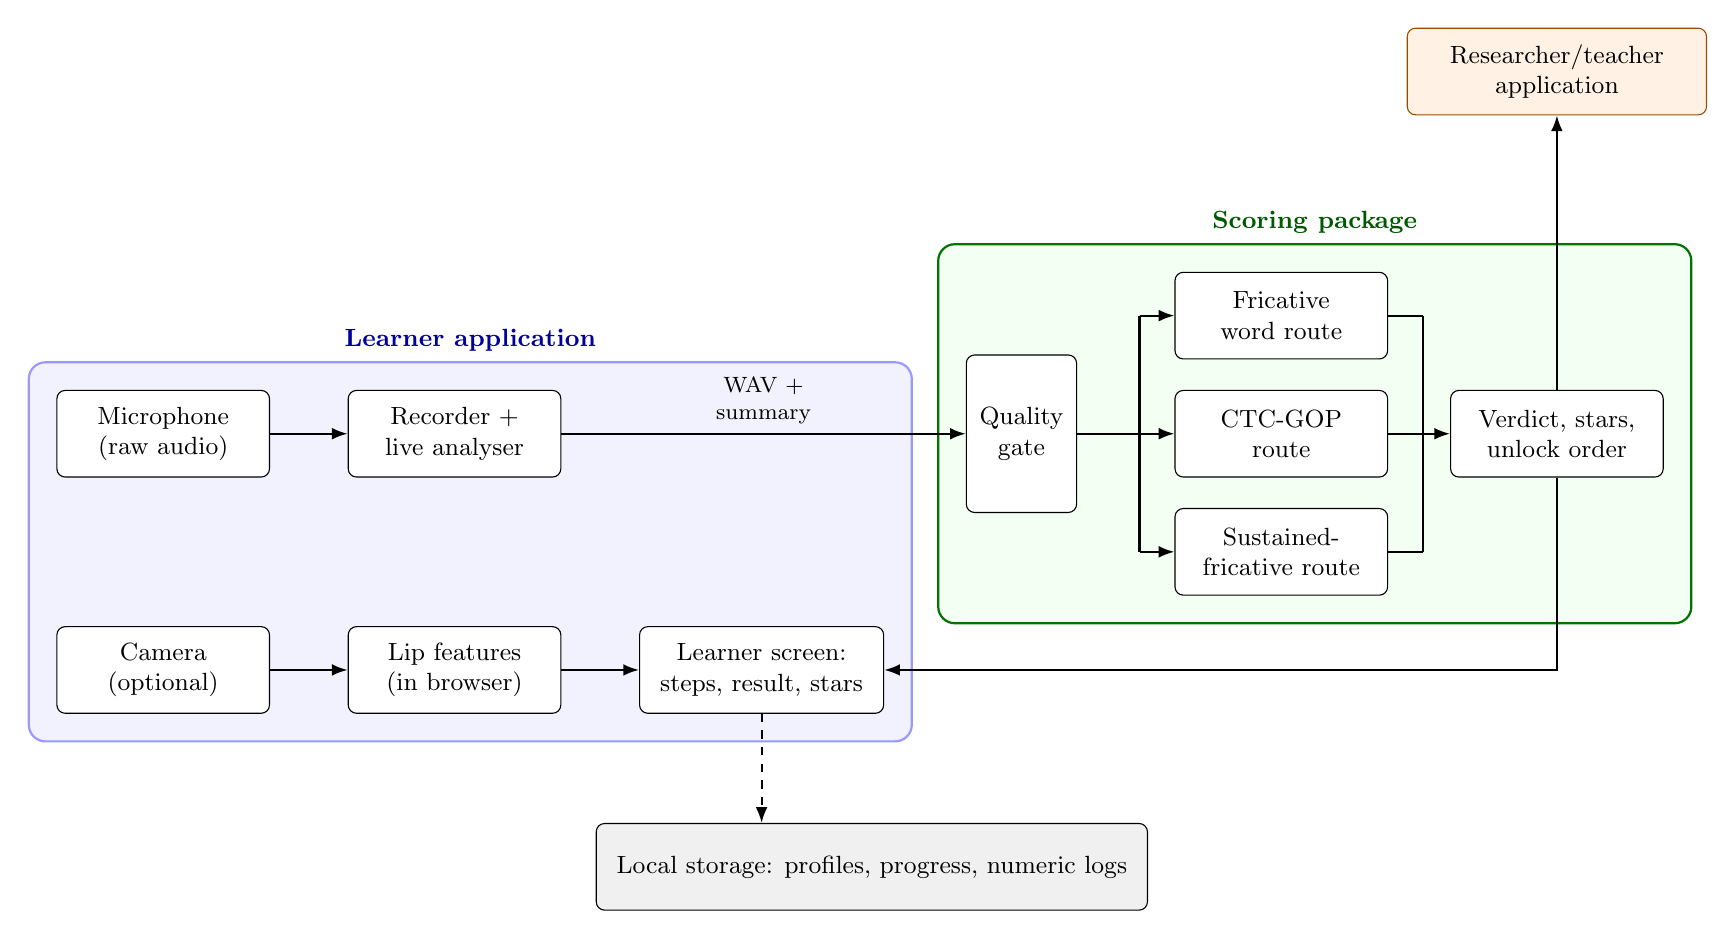
\begin{tikzpicture}[font=\small,
  box/.style={draw, rounded corners=3pt, align=center, fill=white, minimum height=11mm, minimum width=27mm, inner sep=3pt},
  grp/.style={draw, rounded corners=6pt, inner sep=3.5mm, thick},
  arr/.style={-{Latex[length=2mm]}, thick}, bus/.style={thick}]
  \node[box] (mic) at (0,3.6) {Microphone\\(raw audio)};
  \node[box] (cam) at (0,0.6) {Camera\\(optional)};
  \node[box] (rec) at (3.7,3.6) {Recorder +\\live analyser};
  \node[box] (lip) at (3.7,0.6) {Lip features\\(in browser)};
  \node[box, minimum width=31mm] (ui) at (7.6,0.6) {Learner screen:\\steps, result, stars};
  \begin{scope}[on background layer]
    \node[grp, fill=blue!5, draw=blue!40, fit=(mic)(cam)(rec)(lip)(ui), label={[font=\small\bfseries, text=blue!60!black]above:Learner application}] (gA) {};
  \end{scope}
  \node[box, minimum width=14mm, minimum height=20mm] (gate) at (10.9,3.6) {Quality\\gate};
  \node[box] (r1) at (14.2,5.1) {Fricative\\word route};
  \node[box] (r2) at (14.2,3.6) {CTC-GOP\\route};
  \node[box] (r3) at (14.2,2.1) {Sustained-\\fricative route};
  \node[box] (vd) at (17.7,3.6) {Verdict, stars,\\unlock order};
  \begin{scope}[on background layer]
    \node[grp, fill=green!5, draw=green!45!black, fit=(gate)(r1)(r2)(r3)(vd), label={[font=\small\bfseries, text=green!35!black]above:Scoring package}] (gB) {};
  \end{scope}
  \node[box, fill=orange!10, draw=orange!60!black, minimum width=38mm] (dev) at (17.7,8.2) {Researcher/teacher\\application};
  \node[box, fill=gray!12, minimum width=70mm] (st) at (9.0,-1.9) {Local storage: profiles, progress, numeric logs};
  \draw[arr] (mic) -- (rec);
  \draw[arr] (cam) -- (lip);
  \draw[arr] (lip) -- (ui);
  \draw[arr] (rec.east) -- node[above, font=\footnotesize, align=center]{WAV +\\summary} (gate.west |- rec.east);
  \coordinate (b1) at (12.4,3.6);
  \draw[bus] (gate.east) -- (b1); \draw[bus] (b1 |- r1) -- (b1 |- r3);
  \draw[arr] (b1 |- r1) -- (r1.west); \draw[arr] (b1) -- (r2.west); \draw[arr] (b1 |- r3) -- (r3.west);
  \coordinate (b2) at (16.0,3.6);
  \draw[bus] (r1.east) -- (b2 |- r1); \draw[bus] (b2 |- r1) -- (b2 |- r3); \draw[bus] (r3.east) -- (b2 |- r3);
  \draw[bus] (r2.east) -- (b2); \draw[arr] (b2) -- (vd.west);
  \draw[arr] (vd.north) -- (vd.north |- gB.north) -- (dev.south |- gB.north) -- (dev.south);
  \draw[arr] (vd.south) |- (ui.east);
  \draw[arr, dashed] (ui.south) -- (ui.south |- st.north);
\end{tikzpicture}}
\end{adjustwidth}
\caption{System architecture. The learner application records audio and, if the user switches it on, computes lip features in the browser (no camera picture is stored or sent). The scoring package checks recording quality and follows one of three routes according to the task. The researcher/teacher application reads the same recordings and scores. Dashed arrows: data written to the local machine.}
\label{fig:arch}
\end{figure}

\subsection{Related Work}
Visual--acoustic biofeedback is an established clinical technique whose success depends on the comprehension of the representation, the choice of target, and the practice schedule \cite{hitchcock2023}. Spectrographic displays have long been used with deaf speakers: four deaf adolescents improved under both spectrographic and noninstrumental instruction, with an advantage for the spectrogram for some only \cite{ertmermaki2000}, and children aged 6--11 years, with and without hearing impairment, recognised spectrographic cues above chance after familiarisation \cite{ertmer2004}. For listeners with hearing impairment, visual cues contribute more to consonant than to vowel identification \cite{moradi2017,desai2008}. These studies involve small samples and displays the learner must interpret; they do not show that a guided, step-by-step interface supports independent practice.

For error detection, acoustic--phonetic classifiers for frequently mispronounced sounds discriminated correct from incorrect productions, whereas recogniser confidence measures were weaker predictors of phone-level quality \cite{truong2005}. The present design combines both: a recogniser decides which sound was produced, acoustic measures its degree. The recogniser is a wav2vec~2.0 model \cite{baevski2020} fine-tuned for multilingual phone recognition \cite{xu2022}; fricatives are characterised by spectral moments \cite{jongman2000}; learner errors come from L2-ARCTIC \cite{zhao2018} and native speech from CMU ARCTIC \cite{kominek2004}. \tbd{Add CAPT and GOP primary references and UDL literature.}

\subsection{The Present Study}
This paper presents SeeSound, a web-based prototype for eight English consonants (\ipa{s}, \ipa{\textesh}, \ipa{f}, \ipa{t\textesh}, \ipa{m}, \ipa{n}, \ipa{p}, \ipa{b}). The scope is word-initial consonant production and guided consonant-to-vowel practice; the camera measures visible lip movements, not tongue position. The paper contributes (1) a prototype that gives learners simplified step-by-step guidance and researchers and teachers detailed analysis; (2) an account of how live cues are combined with task-specific assessment routes, and of what each route can and cannot support; and (3) technical evaluations, with corpus evidence, single-speaker logs, and synthetic-input tests kept apart. Its usability and effectiveness for DHH learners have not yet been established. Section~\ref{sec:methods} describes the system and the evaluation, Section~\ref{sec:results} the results, and Section~\ref{sec:disc} their limits and the planned user evaluation.

\section{Materials and Methods}\label{sec:methods}
\subsection{System Architecture and Learner Workflow}
SeeSound consists of two web applications that share one scoring package (Figure~\ref{fig:arch}). The \emph{learner application} offers a home page, an optional Sound Check, eight lessons, an optional lip mirror, and a page with the stars earned; all text is in English and Traditional Chinese. The \emph{researcher/teacher application} shows the recording, the spectrogram with the detected consonant, the measures, the recogniser's candidate scores and decoded phones, and the logs. Audio is recorded in the browser and sent to a local Python back end; lip features are computed in the browser and only numbers are passed on. In Figure~\ref{fig:arch}, what the child does is on the left, how the result is decided in the middle, and what is shown or stored on the right.


A lesson (Figure~\ref{fig:flow}) shows the word with a picture for its meaning and one for the sound, an articulation illustration with the steps of the movement, a recorder with live feedback and, for seven of the eight sounds (all but \ipa{f}), an optional lip mirror. After a recording, the recorder is replaced by a three-level mark, a written tip, and one to three stars (three for green, two or one for yellow, none for red). A profile keeps the best result for each word. The lessons are ordered \textit{she}, \textit{see}, \textit{fee}, \textit{pea}, \textit{bee}, \textit{me}, \textit{knee}, \textit{cheat}, and a lesson opens when the one before it has at least two stars; without a profile every lesson is open and nothing is saved. This order and the pass line are application rules chosen during development, not a validated sequence of difficulty or a certificate of mastery.

\begin{figure}[!t]
\begin{adjustwidth}{-\extralength}{0cm}
\centering
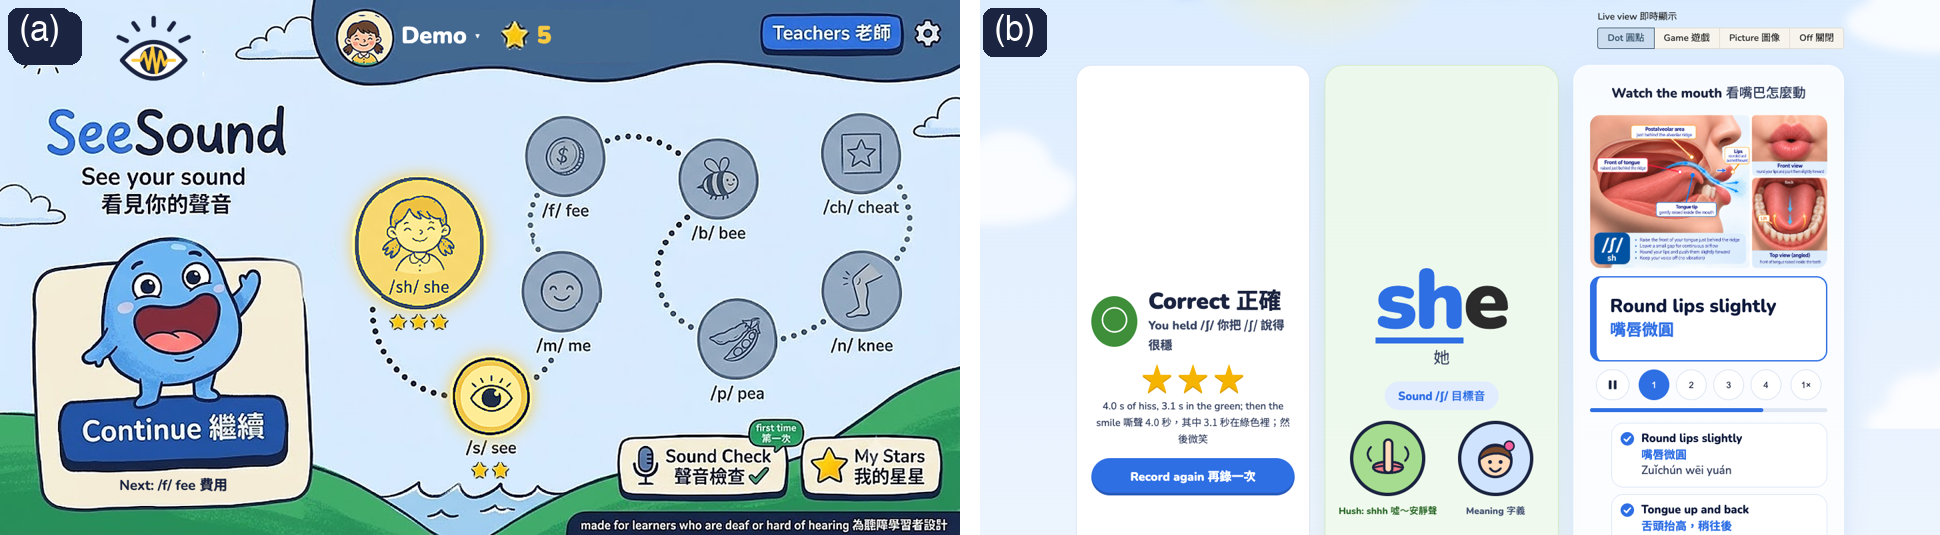
\includegraphics[width=\linewidth]{figs/fig_learner_two.png}
\end{adjustwidth}
\caption{The learner application, run with a test profile and a synthetic microphone signal. (\textbf{a}) Home page: the child's name and stars, the sounds already practised (lit, with their stars), and the button to the next sound. (\textbf{b}) A lesson after a recording: from left to right the result (mark, stars, and the time the hiss spent in the target zone), the word with its two pictures, and the articulation steps.}
\label{fig:flow}
\end{figure}

\subsection{Recording and Live Guidance}
Audio is recorded by a purpose-written component that requests the microphone with echo cancellation, noise suppression, and automatic gain control switched off, and sends mono 16-bit WAV to the back end. Default browser processing clipped the signal and removed the weak onset of \ipa{b} in the first recordings of one adult; switching it off exposes the background noise, so the choice may not suit every room. Table~\ref{tab:tasks} summarises, for each sound, what the child sees while speaking, what the camera checks, and which assessment route produces the result. Recording rules differ between tasks. The word recorder stops after three seconds. The guided recorders listen to the room for 0.6~s, set a sound gate from it, and stop after 1.5~s of silence, at task completion, or after 10--12~s. For \ipa{s} and \ipa{\textesh}, the child holds a hiss in a target zone shown by a moving dot and then smiles into ``ee''; for \ipa{m} and \ipa{n}, the child hums and moves to a vowel; for \ipa{t\textesh}, a train scene follows the pop, the hiss, and the voice (Figure~\ref{fig:live}). Before scoring, a quality gate refuses recordings that clip, are too quiet, or lie less than 12~dB above their own background (lowered from 20~dB after the first recordings; not validated for children).

\begin{figure}[!t]
\centering
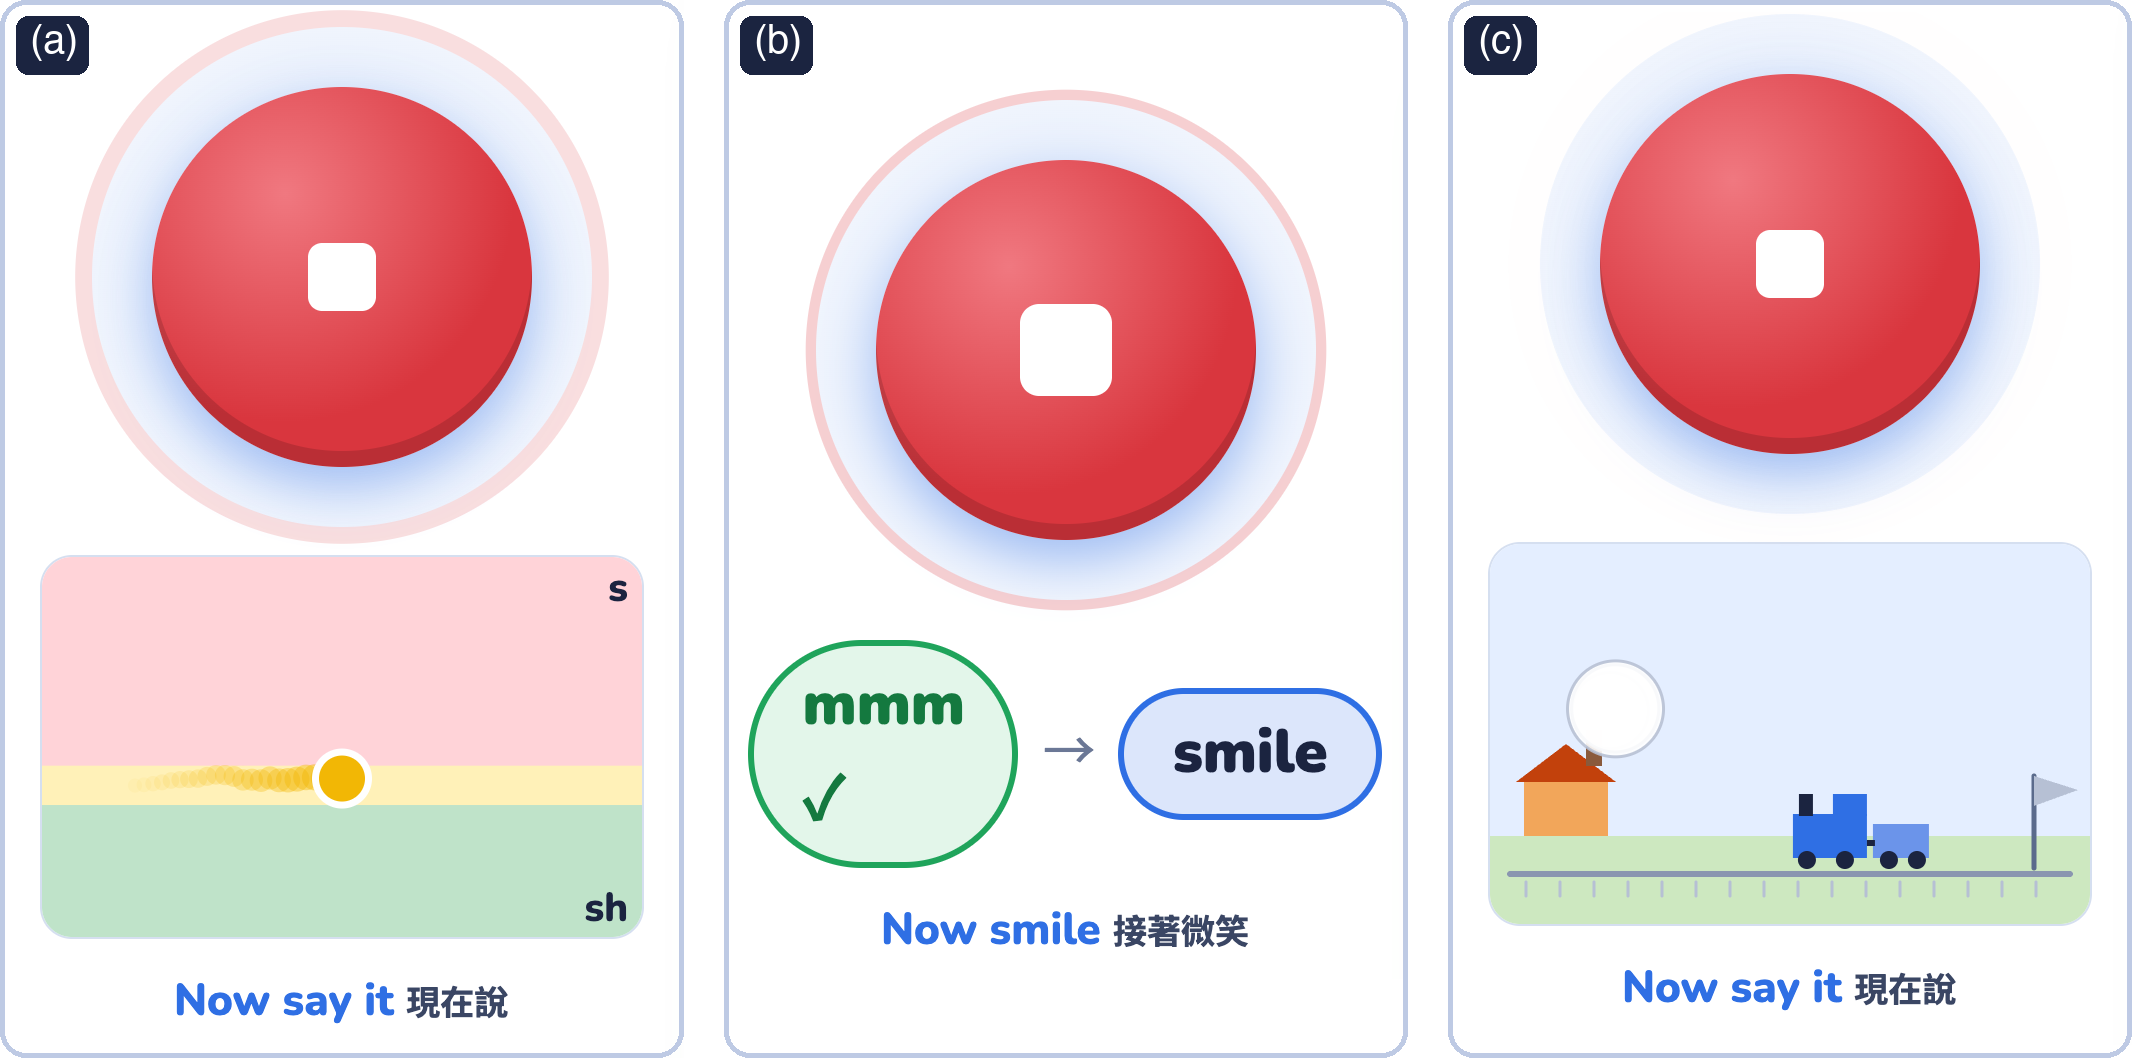
\includegraphics[width=0.5\textwidth]{figs/fig_live.png}
\caption{Live guidance during a recording (red button), driven by synthetic audio. (\textbf{a}) \ipa{\textesh}: the dot has moved into the yellow band while a hiss is held. (\textbf{b}) \ipa{m}: the hum was detected and the smile step is shown. (\textbf{c}) \ipa{t\textesh}: the train reacts to the pop, hiss, and voice.}
\label{fig:live}
\end{figure}

\begin{table}[!t]
\caption{Sounds, tasks and assessment routes. The camera does not see the tongue or the airflow.\label{tab:tasks}}
\small
\begin{tabularx}{\textwidth}{p{1.9cm}p{4.2cm}p{3.3cm}X}
\toprule
\textbf{Sound (word)} & \textbf{Live guidance} & \textbf{Camera cue} & \textbf{Assessment route}\\
\midrule
\ipa{\textesh} (\textit{she}), \ipa{s} (\textit{see}) & Dot/game/spectrogram; hold the hiss in the zone, then ``ee'' & Ghost mouth, three steps & Sustained-fricative route; word route without a live summary\\
\ipa{f} (\textit{fee}) & Level meter relative to the child's ``aaa'' & None & Fricative word route\\
\ipa{p} (\textit{pea}), \ipa{b} (\textit{bee}) & None while speaking & Lips closed, open, spread (camera only) & CTC-GOP\\
\ipa{m} (\textit{me}), \ipa{n} (\textit{knee}) & Hum, then vowel; coach with lips & Lips closed (\ipa{m}) or slightly open (\ipa{n}), then smile & CTC-GOP\\
\ipa{t\textesh} (\textit{cheat}) & Train: pop, hiss, voice & Ghost mouth, three steps & CTC-GOP plus two lamps (pop slope, hiss length)\\
\bottomrule
\end{tabularx}
\end{table}

\subsection{Lip Cues, Sound Check and Data Handling}
When the lip mirror is switched on, a face-landmark model (MediaPipe Face Landmarker, run in the browser from local files) provides two ratios, the inner lip gap and the mouth width, each divided by the forehead-to-chin distance. Lips count as together below a gap ratio of 0.03, and a smile is a width of at least 1.03 times that child's closed-lip width; these limits are first guesses from one adult face. No camera picture is shown, stored, or sent. Sound Check measures the room and asks the child to say a long ``aaa'' twice; the median third formant, relative to a reference of 2625~Hz and limited to 0.85--1.5, shifts the \ipa{s}--\ipa{\textesh} boundary. It was checked on synthetic vowels only, so it is a provisional scaling. The learner application logs numbers and choices only and keeps no audio of the child. Consent and deletion procedures must be defined before use with children \tbd{ethical approval}.


\subsection{Assessment Routes}
What counts as a ``correct'' attempt depends on the task. The application therefore uses three routes (Table~\ref{tab:tasks}): one for fricatives said in a word, one for sounds scored by a phone recogniser, and one for a held hiss.

\subsubsection{Fricative Word Route}
For fricatives, the onset is the start of the run of 2.5--12~kHz energy at least 15~dB above the recording's noise floor, and the offset is the first voiced frame. The centre of gravity (CoG) is computed on the middle 50\% with a rectangular window and spectral power two, the setting of the manual Praat reference values. A phone recogniser (wav2vec~2.0 XLSR-53 fine-tuned on eSpeak phones \cite{baevski2020,xu2022}) decides whether the intended sound was produced, and the acoustic measures decide between \textit{correct} and \textit{almost}; a different sound heard gives \textit{not yet}. It is used for \ipa{f} and for single words with \ipa{s} or \ipa{\textesh}.

\subsubsection{CTC-Based GOP Route}
For \ipa{p}, \ipa{b}, \ipa{m}, \ipa{n}, and \ipa{t\textesh}, a goodness-of-pronunciation score is computed from the CTC output of the same recogniser, with no calibration to the learner. The onset is the first frame whose blank probability is below 0.9, and a window of 22 frames (about 0.45~s) starting three frames earlier is analysed. For each candidate consonant $c$ of a confusable set and each single vowel $v$, the CTC likelihood of $[c,v]$ is summed over vowels and spelling variants $V(c)$, so the vowel the learner chose does not matter:
\begin{equation}
P(c)=\frac{L(c)}{\sum_{c'} L(c')},\qquad L(c)=\sum_{v}\sum_{c_i\in V(c)} p_{\mathrm{CTC}}\bigl([c_i,v]\bigr).
\end{equation}
The verdict is \textit{correct} for $P(\text{target})\geq0.80$, \textit{almost} for at least 0.50 when the target is the top candidate, and \textit{not yet} (naming the sound heard) when another candidate reaches 0.60; otherwise nothing is scored. The limits are provisional. $P$ is a normalised score within the confusable set, not a calibrated probability, and the set restricts the errors that can be recognised; for \ipa{t\textesh} the set includes \ipa{d\textyogh} as a variant, so a voicing error cannot be told from a correct production. Without the recogniser model these five sounds are not scored. For \ipa{t\textesh}, two lamps (pop slope, hiss length) may disagree with the GOP verdict.

\subsubsection{Sustained-Fricative Route}
In guided \ipa{s} and \ipa{\textesh} practice, the verdict is made from what the live guide measured, because the word-level rules and the recogniser refused correct sustained hisses. A hiss under 300~ms is not scored; otherwise the time the CoG spent in the target zone, summed over the hiss, gives \textit{correct} from 800~ms, \textit{almost} from 400~ms, and \textit{not yet} below. The route therefore measures completion of the sustained-hiss task, not whether a short word would be judged correct; its limits are guesses.

\subsection{Evaluation Design}
Four kinds of evidence are used, and they are not combined: (i) \emph{corpus experiments}, on CMU ARCTIC \cite{kominek2004} (eight native voices), on L2-ARCTIC \cite{zhao2018} (24 learners with human-annotated substitutions), and on a small dictionary set with manual Praat values; (ii) \emph{development logs} of one adult; (iii) \emph{tests with synthetic input}; and (iv) a \emph{planned user evaluation}, not yet carried out. Corpus consonants were cut from sentences and padded with silence to approximate isolated words, at 16~kHz. Accuracy on native speech is balanced accuracy with leave-one-voice-out testing. On learner speech, two rates are reported with Wilson 95\% intervals: the false-rejection rate (FR), the share of correct productions marked \textit{not yet}, and the detection rate (Det.), the share of annotated substitutions marked \textit{not yet}. A good route has a low FR and a high Det.

\section{Results}\label{sec:results}
\subsection{Fricatives: Native Thresholds Do Not Transfer to Learners}
On the dictionary set, the tool's CoG differed from the manual Praat values by less than 2~Hz, but this concerns two voices only. The question that matters for learners is whether such a rule still works on their speech. Table~\ref{tab:l2} shows that it does not: fixed thresholds rejected 45\% of the correct \ipa{s} and 43\% of the correct \ipa{\textesh} produced by L2 speakers. The recogniser-assisted route lowered these rates to 8\% and 3\% while still catching 100\% and 88\% of the annotated errors. For these two sounds, a decision on the identity of the sound is therefore needed in addition to the acoustic thresholds.

\begin{table}[!t]
\caption{Fricatives in L2-ARCTIC: false rejection of correct productions (FR) and detection of annotated errors (Det.), with Wilson 95\% intervals; $n$ = correct/error tokens. Lower FR and higher Det. are better.\label{tab:l2}}
\small
\begin{tabularx}{\textwidth}{llccc}
\toprule
\textbf{Sound} & \textbf{Scoring} & \textbf{$n$} & \textbf{FR (correct)} & \textbf{Det. (errors)}\\
\midrule
\multirow{2}{*}{\ipa{s}} & Thresholds & 861/18 & 45\% [42, 49] & 83\% [61, 94]\\
 & Recogniser-assisted & & 8\% [6, 10] & 100\% [82, 100]\\
\multirow{2}{*}{\ipa{\textesh}} & Thresholds & 602/32 & 43\% [39, 47] & 84\% [68, 93]\\
 & Recogniser-assisted & & 3\% [2, 5] & 88\% [72, 95]\\
\bottomrule
\end{tabularx}
\end{table}

\ipa{f} is the exception: the contrast with \ipa{\texttheta} could not be established from the consonant alone (recogniser accuracy 0.99 on whole words, 0.67 on the hiss alone), so this pair is not graded.

\subsection{Other Sounds and the Replaced Probes}
On native speech, a recogniser-based probe clearly beat a hand-crafted acoustic rule for \ipa{m}--\ipa{n} (balanced accuracy 0.98 against 0.63 for Praat formants), \ipa{p}--\ipa{b} (0.96 against 0.88 for a 30~ms voice-onset-time rule), and \ipa{t\textesh}--\ipa{\textesh} (0.96 against 0.80). These probes were evaluated on L2-ARCTIC, but the application now scores these sounds with the GOP route, which has \emph{not} been evaluated against independent labels; learner errors are too few for \ipa{f}, \ipa{m}, \ipa{n}, and \ipa{t\textesh} to report detection rates. The numbers therefore show that a recogniser is a promising basis, not how accurate the current GOP route is.

On 53 development recordings of one adult, the GOP route judged \ipa{t\textesh} \textit{correct} in 5 of 8 recordings, \ipa{m} in 3 of 7, \ipa{n} in 4 of 9, and \ipa{p} in 2 of 8, but \ipa{b} \textit{not yet} in 12 of 21. These are counts of verdicts, not accuracies, because no independent label exists. They show where the route is least stable: the recogniser often heard \ipa{b} before \ipa{a}, \ipa{u} or a schwa as \ipa{m}, and \ipa{m} before \ipa{u} as \ipa{n}. A second recogniser did not do better and was dropped.


\subsection{Live Cues for the Moving Dot}
The live dot and the offline measure compute the CoG differently, so each was checked for how well it separates \ipa{s} from \ipa{\textesh}. Table~\ref{tab:cog} compares three measures on 7104 tokens of four adult ARCTIC voices. The measure chosen for the dot (power-weighted, 2--8~kHz) reaches an AUC of 0.86, between the first version of the dot (0.76) and the offline measure (0.92). The thresholds were chosen on the same tokens, so the figures are exploratory, and the dot still separates the two sounds wrongly about once in four attempts: it is a guide for practice, not an assessment. For \ipa{t\textesh}, in two voices the steepest rise of the hiss envelope separated it from \ipa{\textesh} (AUC 0.83 and 0.87) and the hiss length separated it from \ipa{t} (0.89 and 0.91), but the best limits differed strongly between voices.

\begin{table}[!t]
\caption{Separation of \ipa{s} and \ipa{\textesh} by three CoG measures (7104 tokens, four adult voices); AUC 0.5 is chance, 1.0 is perfect separation.\label{tab:cog}}
\small
\begin{tabularx}{\textwidth}{Xcc}
\toprule
\textbf{Measure} & \textbf{Pooled AUC} & \textbf{Per-voice AUC}\\
\midrule
Amplitude-weighted, 1--8~kHz (first dot) & 0.76 & 0.71--0.89\\
Power-weighted, 2--8~kHz (live dot, chosen) & 0.86 & 0.84--0.91\\
Power-weighted, whole spectrum (offline) & 0.92 & 0.90--0.95\\
\bottomrule
\end{tabularx}
\end{table}

\section{Discussion}\label{sec:disc}
\textbf{Main finding.} Validation on native speech is not sufficient for an assistive tool: a measure that agrees with expert manual measurement can still reject many correct learner productions (Table~\ref{tab:l2}), and the unit of evaluation changes the conclusion about a recogniser (the \ipa{f}--\ipa{\texttheta} case).

\textbf{Design questions that remain.} The three routes answer different questions: success in the sustained-fricative route does not show that a short word would be judged correct, and a child may see a live lamp that disagrees with the later verdict, so a policy for such conflicts is needed. Recording rules also differ between tasks; one procedure for all lessons would make recordings easier to compare in a study run by teachers. Finally, the camera shows only visible lip movements, and for \ipa{p} and \ipa{b} the lip steps can be completed without any sound.

\textbf{Limitations.} No DHH learner has used the tool, and the corpus learners are hearing speakers, so the findings cannot be generalised to DHH speech. Corpus consonants were cut from sentences, and annotated errors are few for several sounds. All limits (GOP, lip ratios, hold times, quality gate, the two-star pass line, voice-size factor) were set on small data, mainly from one adult. The Chinese interface texts have not been reviewed by a native-speaking educator. Learning outcomes have not been measured, and stars and lesson order are not evidence of mastery.

\textbf{Planned user evaluation.} Experts (phoneticians, speech-language pathologists, teachers of DHH learners) will first review the illustrations, tips, lesson order, and feedback. In a learner strand, at least two teachers blind to the tool's verdicts will rate each target consonant, and tool--teacher agreement will be compared with teacher--teacher agreement for each route, with unscored attempts reported; usability measures include step completion and understanding of the colours. Learning outcomes belong to a later stage. \tbd{Numbers, recruitment, instruments, ethical approval, consent.}

\section{Conclusions}
SeeSound, a prototype with a learner interface and a researcher/teacher interface for eight English consonants, was described and evaluated technically. On annotated learner speech, a recogniser-assisted route reduced false rejection of \ipa{s} and \ipa{\textesh} to 8\% and 3\% without losing the annotated confusions, a live CoG indicator separated the two sounds with an AUC of 0.86, and the \ipa{f}--\ipa{\texttheta} contrast could not be established from the consonant alone. The GOP and sustained-fricative routes have been tested for function but not against independent labels. The prototype is intended to support independent practice by DHH children after initial guidance and teacher-led intervention; whether it does so remains to be shown. Future work: isolated words from native, L2, and DHH speakers, evaluation of each route against independent ratings, expert review of the content, and measurement of usability and learning.

\vspace{6pt}
\authorcontributions{\tbd{Conceptualization, software, writing: K.P., Q.N.; supervision: H.-K.S.}}
\funding{\tbd{FTIP project, National Formosa University; grant number}}
\institutionalreview{\tbd{Not applicable for this technical study / approval for later user studies}}
\informedconsent{\tbd{}}
\dataavailability{\tbd{Code and corpus-evaluation scripts; the corpora are public}}
\conflictsofinterest{The authors declare no conflicts of interest.}

\reftitle{References}
\begin{thebibliography}{999}
\bibitem{ertmer2011} Ertmer, D.J.; Goffman, L. Speech production accuracy and variability in young cochlear implant recipients: Comparisons with typically developing age-peers. {\em J. Speech Lang. Hear. Res.} {\bf 2011}, {\em 54}, 177--189.
\bibitem{stelmachowicz2004} Stelmachowicz, P.G.; Pittman, A.L.; Hoover, B.M.; Lewis, D.E.; Moeller, M.P. The importance of high-frequency audibility in the speech and language development of children with hearing loss. {\em Arch. Otolaryngol. Head Neck Surg.} {\bf 2004}, {\em 130}, 556--562.
\bibitem{hitchcock2023} Hitchcock, E.R.; Ochs, L.C.; Swartz, M.T.; Leece, M.C.; Preston, J.L.; McAllister, T. Tutorial: Using visual--acoustic biofeedback for speech sound training. {\em Am. J. Speech-Lang. Pathol.} {\bf 2023}, {\em 32}, 18--36.
\bibitem{bu2021} Bu, Y.; et al. PTeacher: A computer-aided personalized pronunciation training system with exaggerated audio-visual corrective feedback. In Proc. CHI '21; 2021; pp. 1--14.
\bibitem{neri2006} Neri, A.; Cucchiarini, C.; Strik, H. ASR-based corrective feedback on pronunciation: Does it really work? In Proc. Interspeech; 2006.
\bibitem{ertmermaki2000} Ertmer, D.J.; Maki, J.E. A comparison of speech training methods with deaf adolescents: Spectrographic versus noninstrumental instruction. {\em J. Speech Lang. Hear. Res.} {\bf 2000}, {\em 43}, 1509--1523.
\bibitem{ertmer2004} Ertmer, D.J. How well can children recognize speech features in spectrograms? Comparisons by age and hearing status. {\em J. Speech Lang. Hear. Res.} {\bf 2004}, {\em 47}, 484--495.
\bibitem{moradi2017} Moradi, S.; Lidestam, B.; Danielsson, H.; Ng, E.H.N.; R{\"o}nnberg, J. Visual cues contribute differentially to audiovisual perception of consonants and vowels in improving recognition and reducing cognitive demands in listeners with hearing impairment using hearing aids. {\em J. Speech Lang. Hear. Res.} {\bf 2017}, {\em 60}, 2687--2703.
\bibitem{desai2008} Desai, S.; Stickney, G.; Zeng, F.-G. Auditory-visual speech perception in normal-hearing and cochlear-implant listeners. {\em J. Acoust. Soc. Am.} {\bf 2008}, {\em 123}, 428--440.
\bibitem{truong2005} Truong, K.; Neri, A.; de Wet, F.; Cucchiarini, C.; Strik, H. Automatic detection of frequent pronunciation errors made by L2-learners. In Proc. Interspeech; 2005.
\bibitem{baevski2020} Baevski, A.; Zhou, Y.; Mohamed, A.; Auli, M. wav2vec 2.0: A framework for self-supervised learning of speech representations. In Proc. NeurIPS; 2020; Volume 33, pp. 12449--12460.
\bibitem{xu2022} Xu, Q.; Baevski, A.; Auli, M. Simple and effective zero-shot cross-lingual phoneme recognition. In Proc. Interspeech; 2022; pp. 2113--2117.
\bibitem{jongman2000} Jongman, A.; Wayland, R.; Wong, S. Acoustic characteristics of English fricatives. {\em J. Acoust. Soc. Am.} {\bf 2000}, {\em 108}, 1252--1263.
\bibitem{zhao2018} Zhao, G.; et al. L2-ARCTIC: A non-native English speech corpus. In Proc. Interspeech; 2018; pp. 2783--2787.
\bibitem{kominek2004} Kominek, J.; Black, A.W. The CMU Arctic speech databases. In Proc. SSW 5; 2004; pp. 223--224.
\end{thebibliography}

\end{document}
